% Beamer Presentation and Lecture Note Template
% Version 0.1
% by Paul Vesey

\mode<presentation> {
\usetheme{Antibes}
\setbeamercovered{invisible}
\setbeamertemplate{footline}[frame number]
\setbeamertemplate{navigation symbols}{} 
}

\usepackage{eurosym}
\usepackage{graphicx}
\usepackage{wasysym}
\usepackage{hyperref}
\usepackage{amsmath}
\usepackage{amssymb}
\usepackage{mathtools}
\usepackage{tikz}
\usepackage{pgf}
\usepackage{pgfplots}
\usepackage{pxfonts}
\usepackage{textcomp}
\usepackage{verbatim}
\usepackage{color}
\usepackage{xcolor}
\usepackage{fix-cm}


\author{Paul Vesey}
\institute[LIT]
{
Limerick Institute of Technology \\
\medskip
{\emph{paul.vesey@lit.ie}}
}
\date{Spring 2021}



%\usepackage{bm} 
% For typesetting bold math (not \mathbold)
%\logo{\includegraphics[height=0.6cm]{yourlogo.eps}}
%
\title[Building Information Modelling]{Building Information Modelling}


\begin{document}
%
\usetikzlibrary{arrows}
\usepgflibrary{patterns}



\thispagestyle{empty} % Remove page numbering on this page

%----------------------------------------------------------------------------------------
%	TITLE SECTION
%----------------------------------------------------------------------------------------

\hrule

\vspace*{0.7cm} % Space between the start of the title and the top of the grey box


\begin{flushright}
\Huge Construction Project Management \\
\vspace*{0.7cm}
\Large Certificate in Construction Project Management\\
Autumn 2020
\end{flushright}

\vspace*{0.7cm} % Space between the end of the title and the bottom of the grey box
	
\normalsize

\hrule

%----------------------------------------------------------------------------------------

\vfill % Space between the title box and author information

%----------------------------------------------------------------------------------------
%	AUTHOR NAME AND INFORMATION SECTION
%----------------------------------------------------------------------------------------

{\centering \large 
\hfill Paul Vesey, \scriptsize BEng (Hons), MIE, HDip\normalsize \\
\hfill Limerick Institute of Technology \\
\hfill Department of the Built Environment \\
\hfill \texttt{https://www.lit.ie} \\
\vspace*{0.7cm} 
\hrule} % Horizontal line, thickness changed here

%----------------------------------------------------------------------------------------

\clearpage % Whitespace to the end of the page

\newpage




\thispagestyle{empty}
\tableofcontents
\newpage
\section{Introduction}


\begin{frame}
\titlepage
\end{frame}\begin{center}\line(1,0){250}\end{center}
%
%
\begin{center}\line(1,0){250}\end{center}




\section{Introduction to PAS 1192}

\begin{frame}
\frametitle{}
\begin{figure}
	\centering
	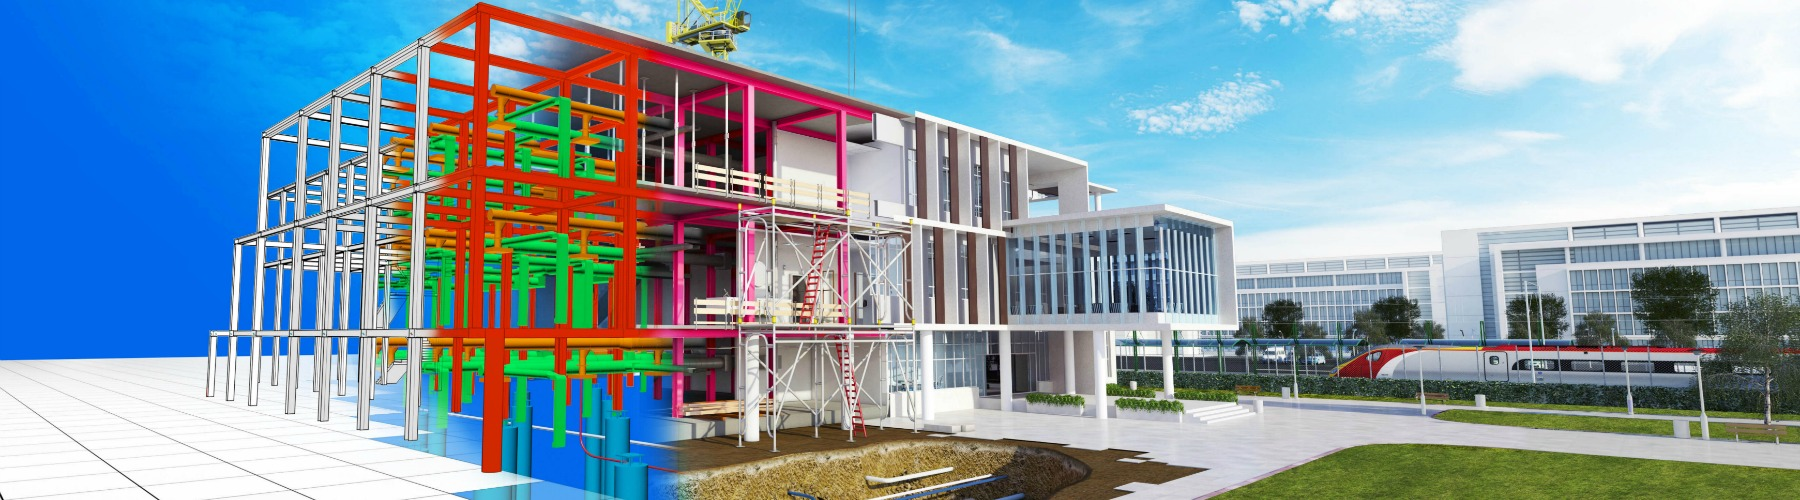
\includegraphics[width=10cm]{./images/bim-banner-bg-1.jpg}
	\caption[]{}
	\label{fig:}
\end{figure}
\begin{itemize}
	\item 
\end{itemize}
\end{frame}
\begin{center}\line(1,0){250}\end{center}






\begin{frame}
\frametitle{}
\begin{figure}
	\centering
	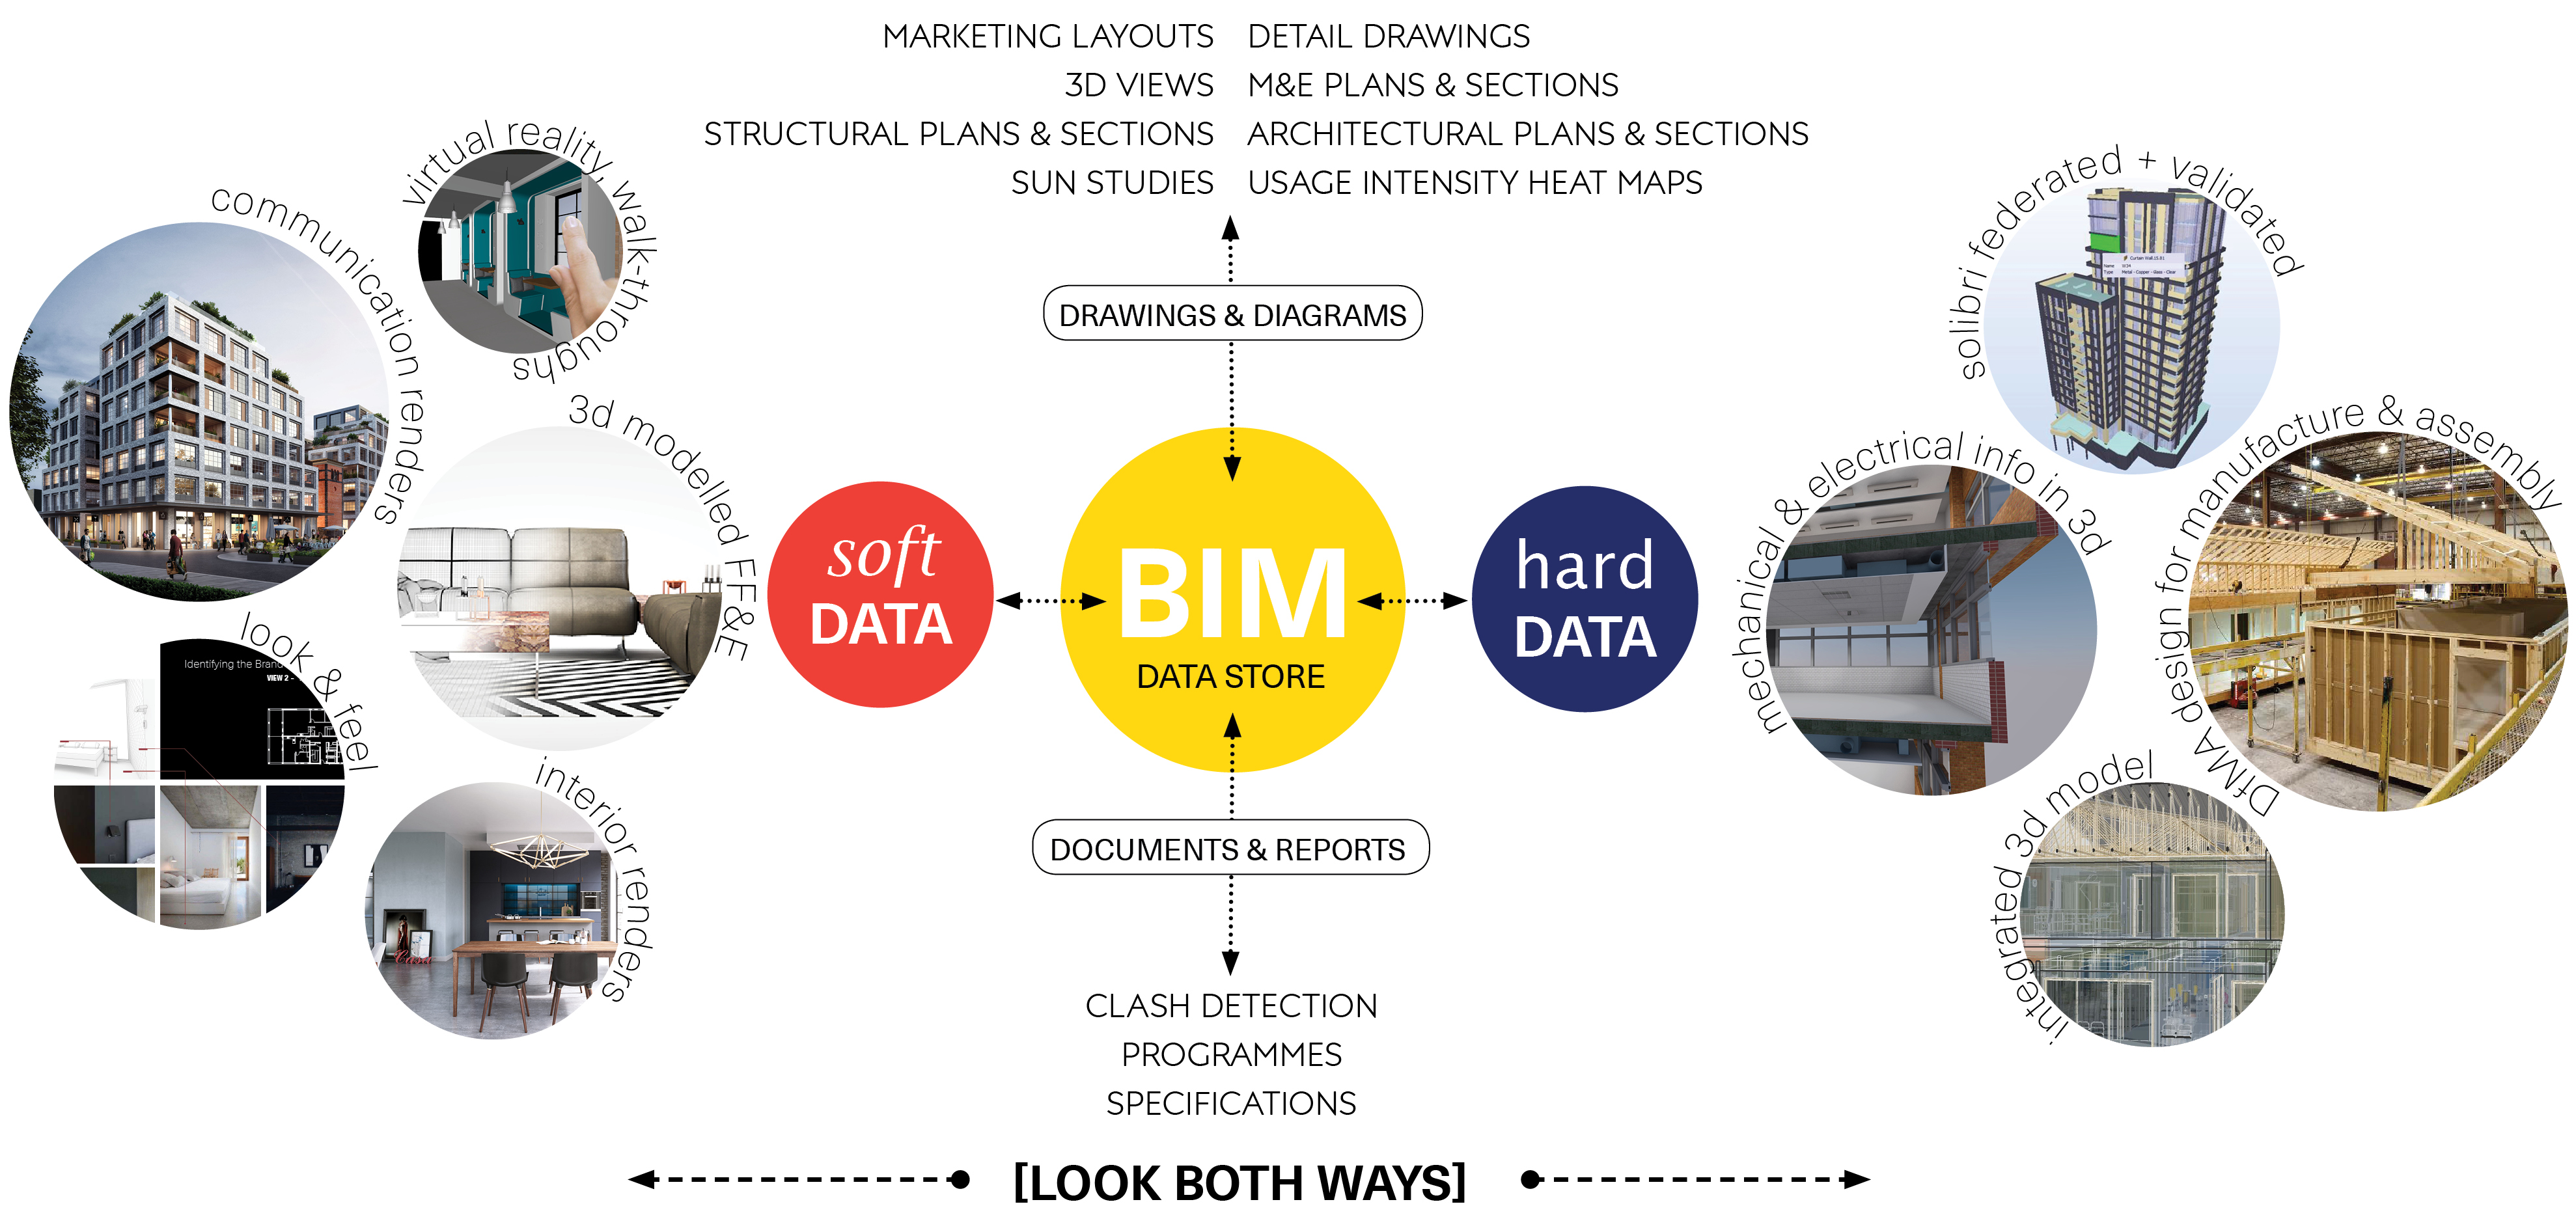
\includegraphics[width=10cm]{./images/BIM-Data-Store-4.jpg}
	\caption[]{}
	\label{fig:}
\end{figure}
\begin{itemize}
	\item 
\end{itemize}
\end{frame}
\begin{center}\line(1,0){250}\end{center}




\begin{frame}
\frametitle{}
\begin{figure}
	\centering
	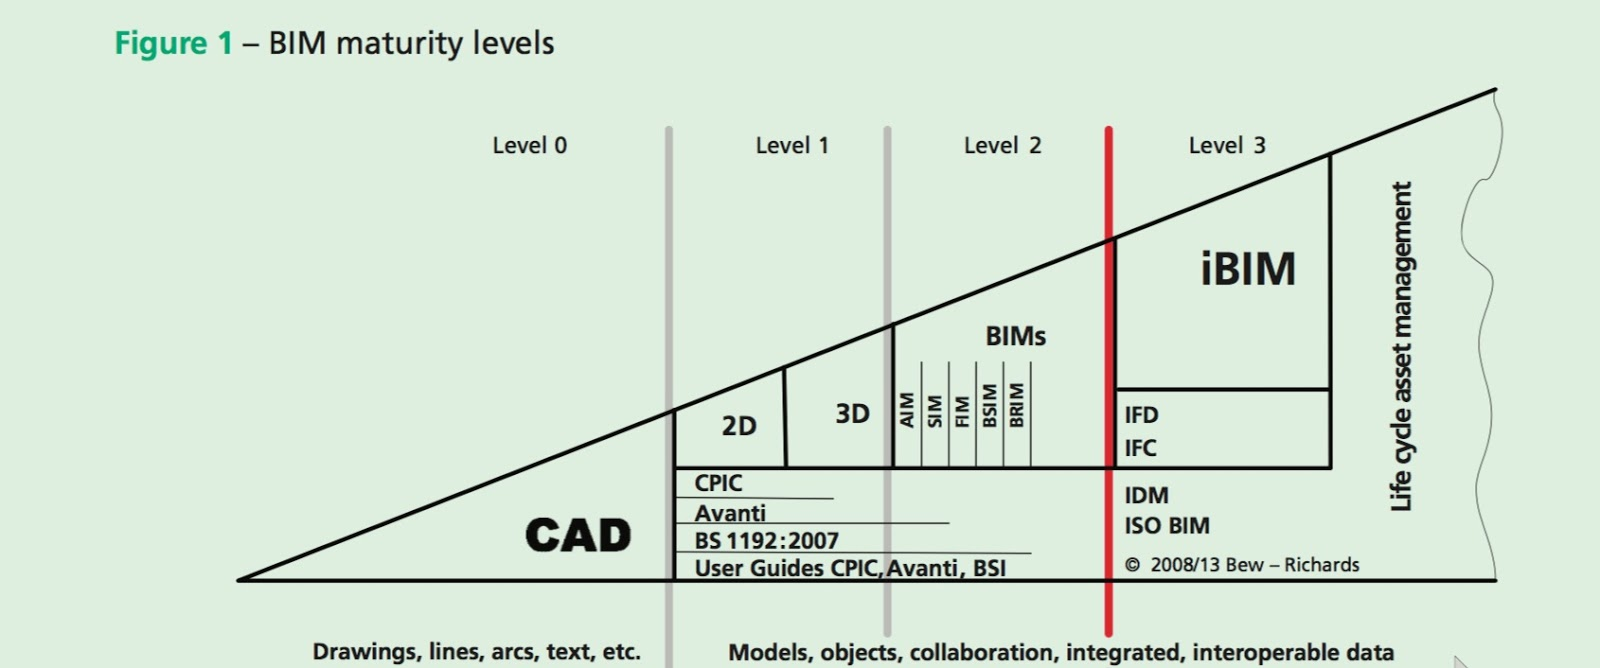
\includegraphics[width=10cm]{./images/bimmaturity Levels.jpg}
	\caption[]{}
	\label{fig:}
\end{figure}
\begin{itemize}
	\item 
\end{itemize}
\end{frame}
\begin{center}\line(1,0){250}\end{center}



\begin{frame}
\frametitle{}
\begin{figure}
	\centering
	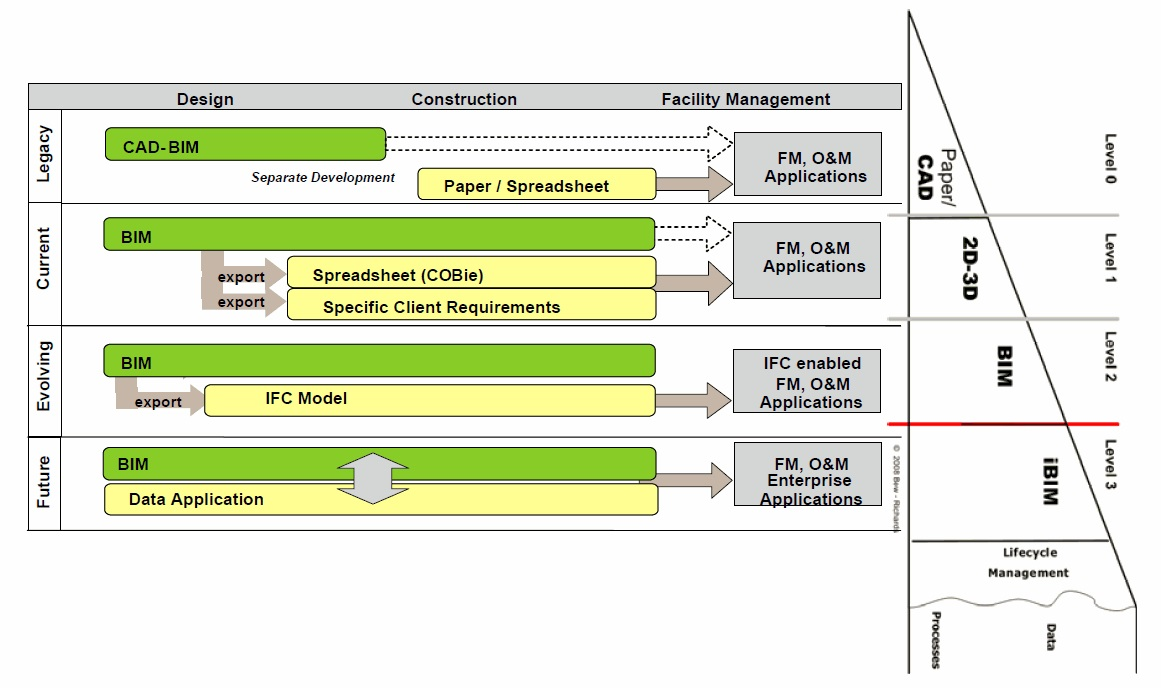
\includegraphics[width=10cm]{./images/COBie-levels.jpg}
	\caption[]{}
	\label{fig:}
\end{figure}
\begin{itemize}
	\item 
\end{itemize}
\end{frame}
\begin{center}\line(1,0){250}\end{center}



\begin{frame}
\frametitle{}
\begin{figure}
	\centering
	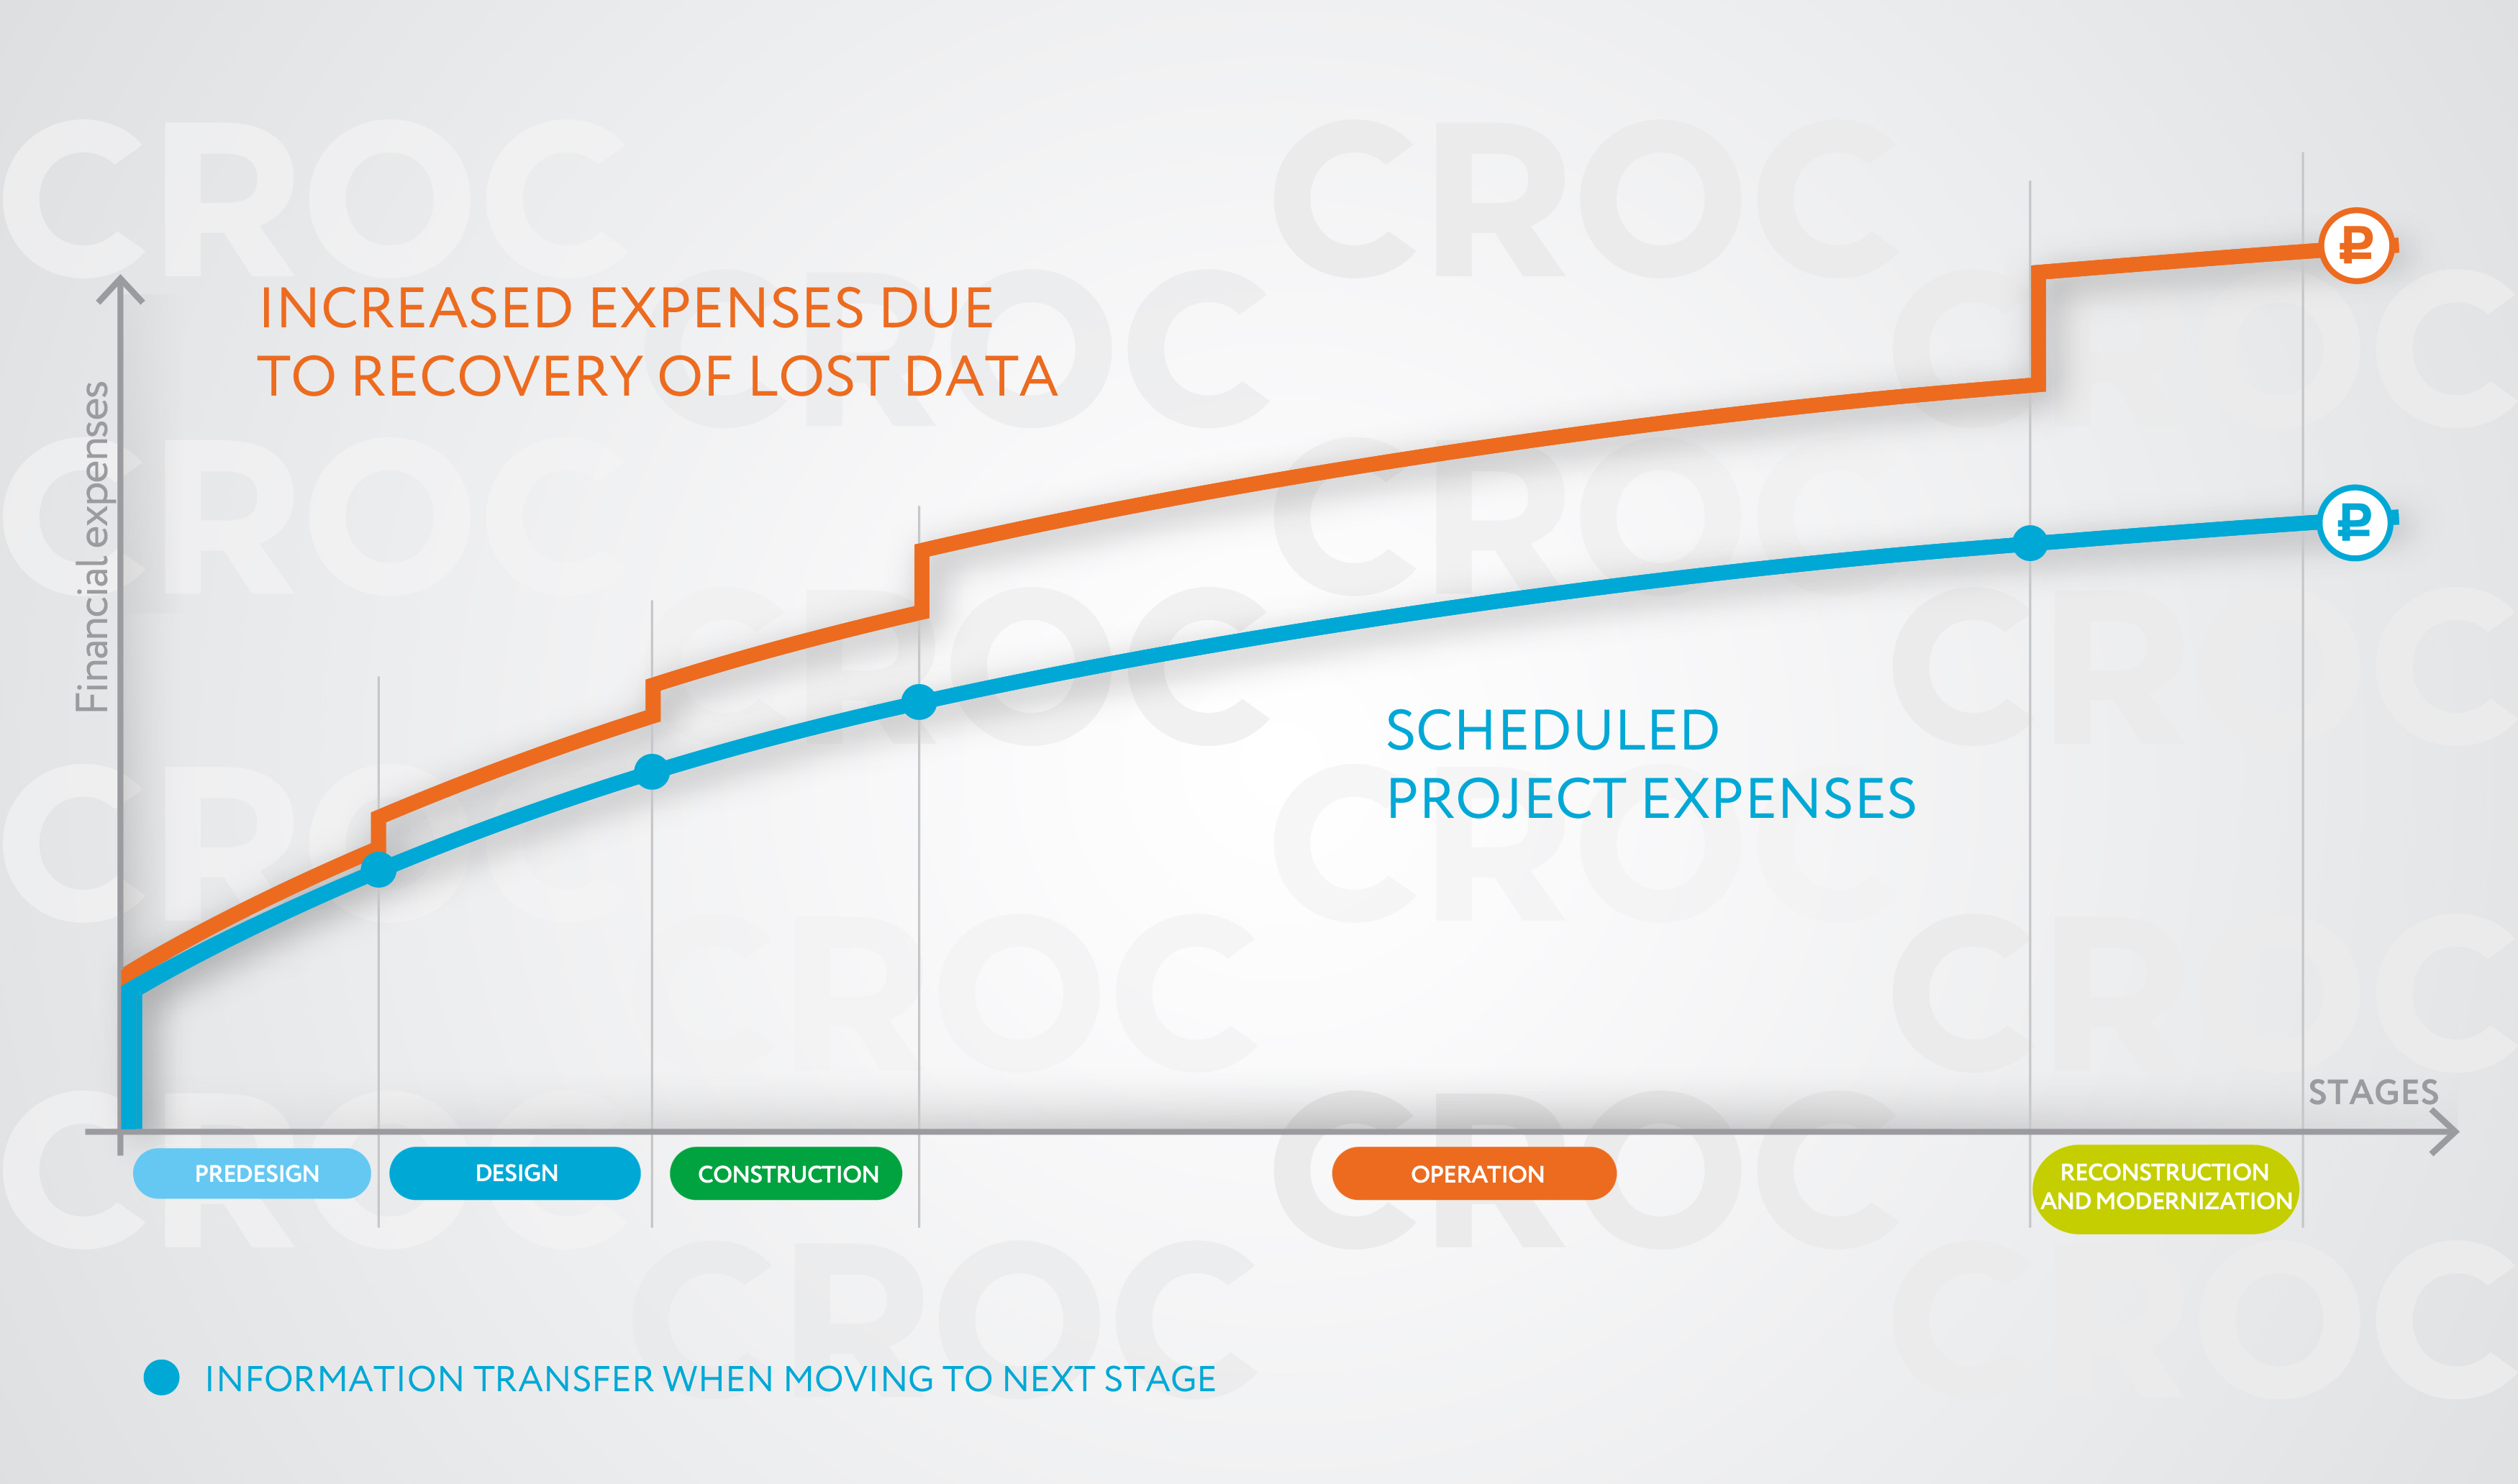
\includegraphics[width=10cm]{./images/InformationTransferCost.jpg}
	\caption[]{}
	\label{fig:}
\end{figure}
\begin{itemize}
	\item 
\end{itemize}
\end{frame}
\begin{center}\line(1,0){250}\end{center}





\begin{frame}
\frametitle{}
\begin{figure}
	\centering
	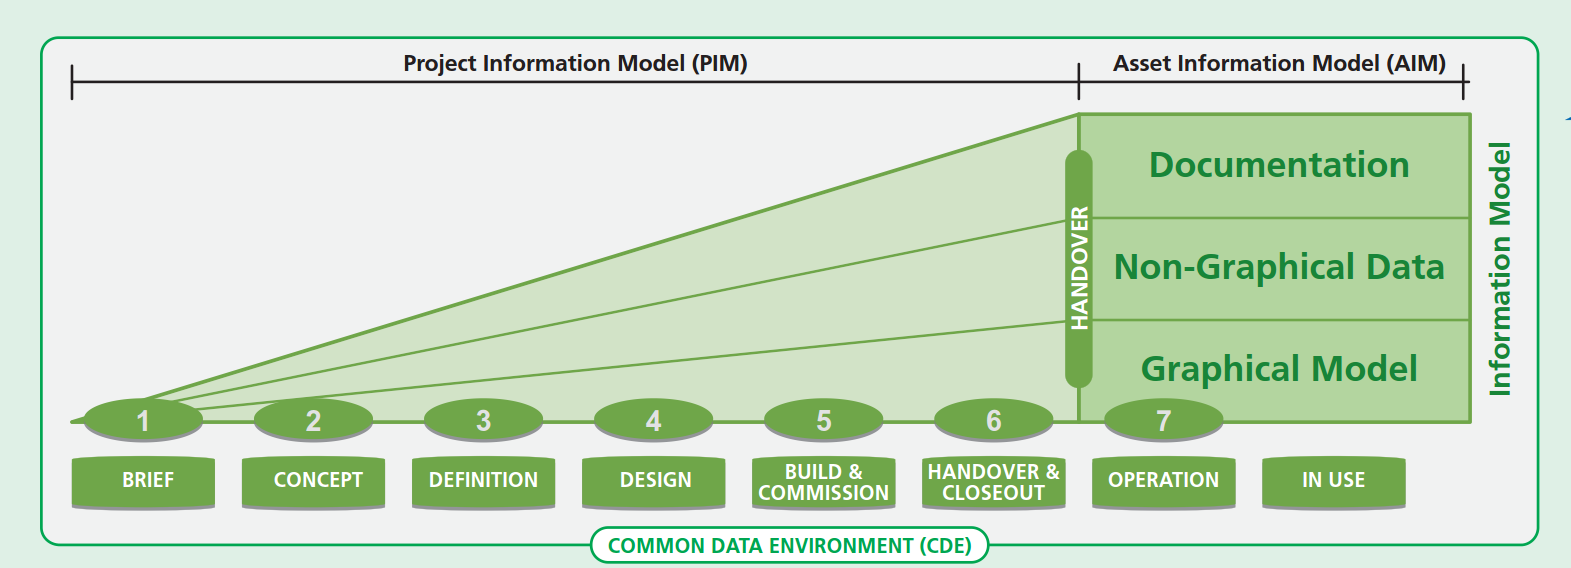
\includegraphics[width=10cm]{./images/Levels-of-Definition-with-BIM-1.png}
	\caption[]{}
	\label{fig:}
\end{figure}
\begin{itemize}
	\item 
\end{itemize}
\end{frame}
\begin{center}\line(1,0){250}\end{center}






\begin{frame}
\frametitle{}
\begin{figure}
	\centering
	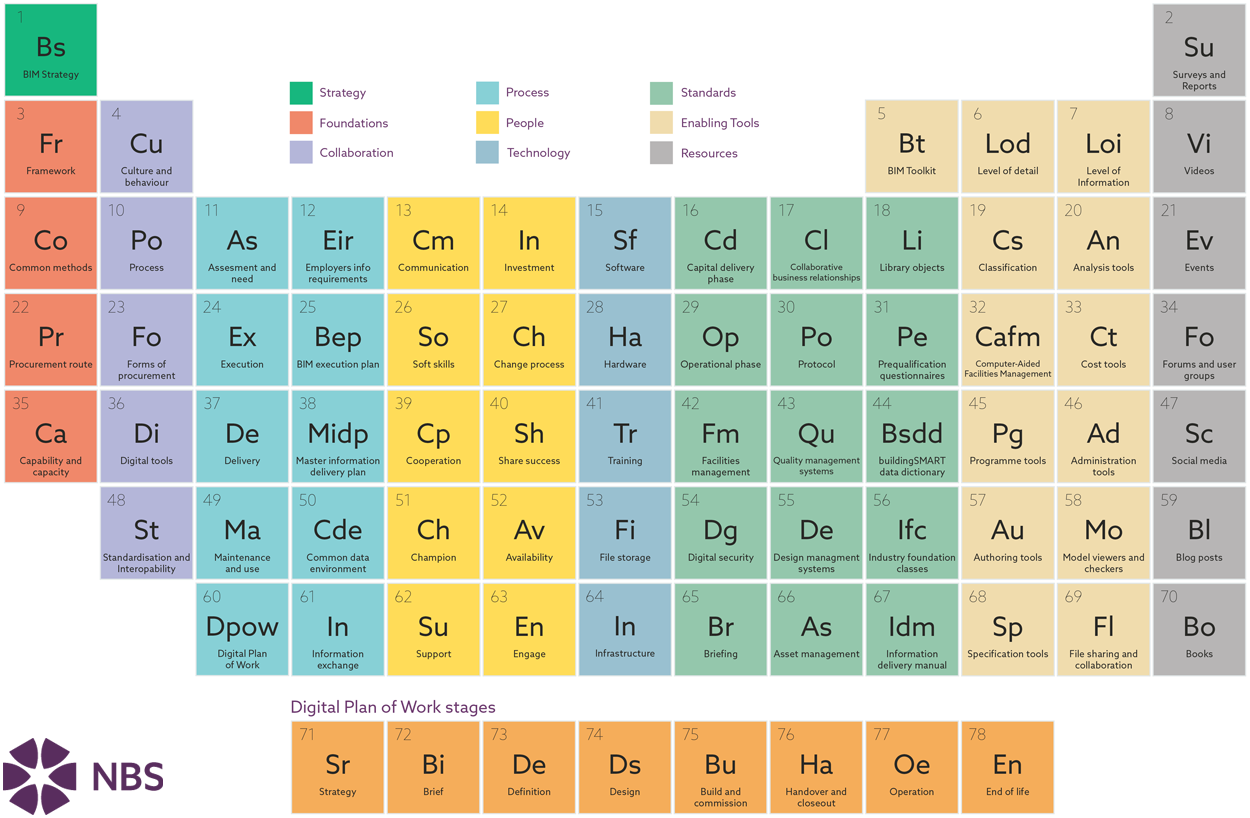
\includegraphics[width=10cm]{./images/nbs-periodic-table-of-bim1.png}
	\caption[]{}
	\label{fig:}
\end{figure}
\begin{itemize}
	\item 
\end{itemize}
\end{frame}
\begin{center}\line(1,0){250}\end{center}


\begin{frame}
\frametitle{}
\begin{figure}
	\centering
	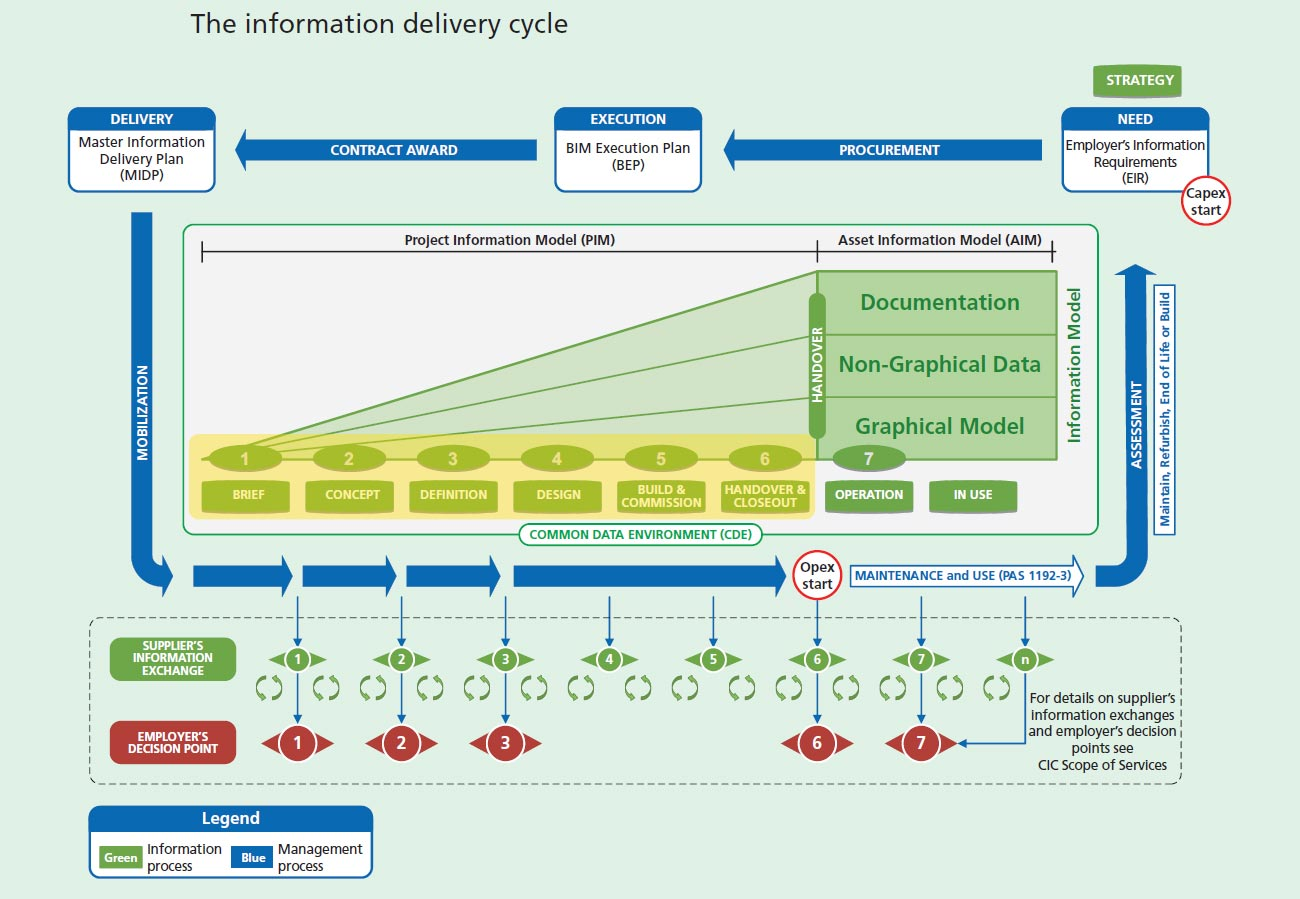
\includegraphics[width=10cm]{./images/Pas-1192-2-2013.jpg}
	\caption[]{}
	\label{fig:}
\end{figure}
\begin{itemize}
	\item 
\end{itemize}
\end{frame}
\begin{center}\line(1,0){250}\end{center}


\begin{frame}
\frametitle{}
\begin{figure}
	\centering
	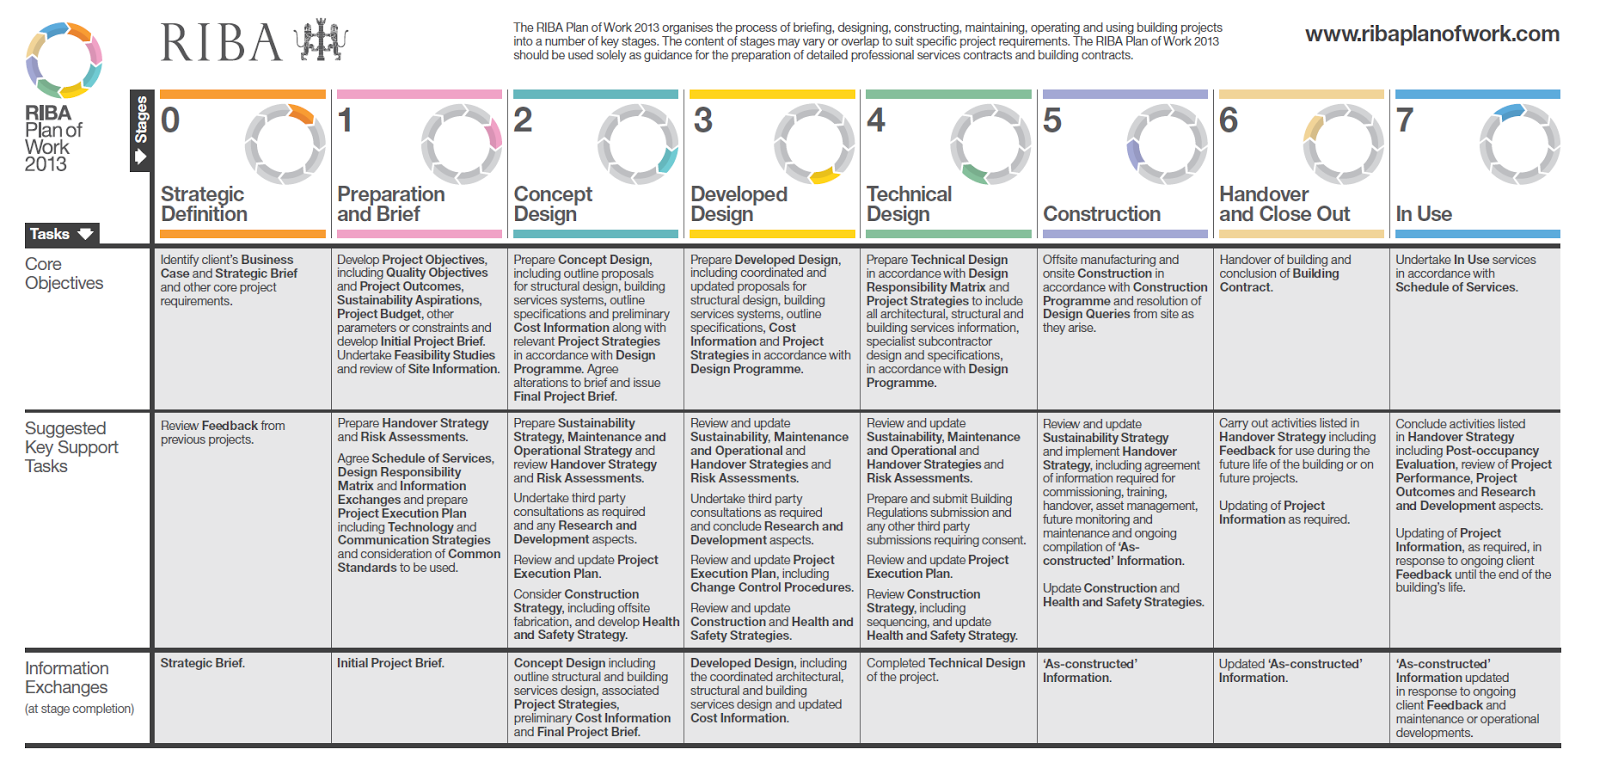
\includegraphics[width=10cm]{./images/RIBAPlanofworkstable.png}
	\caption[]{}
	\label{fig:}
\end{figure}
\begin{itemize}
	\item 
\end{itemize}
\end{frame}
\begin{center}\line(1,0){250}\end{center}


\begin{frame}
\frametitle{}
\begin{figure}
	\centering
	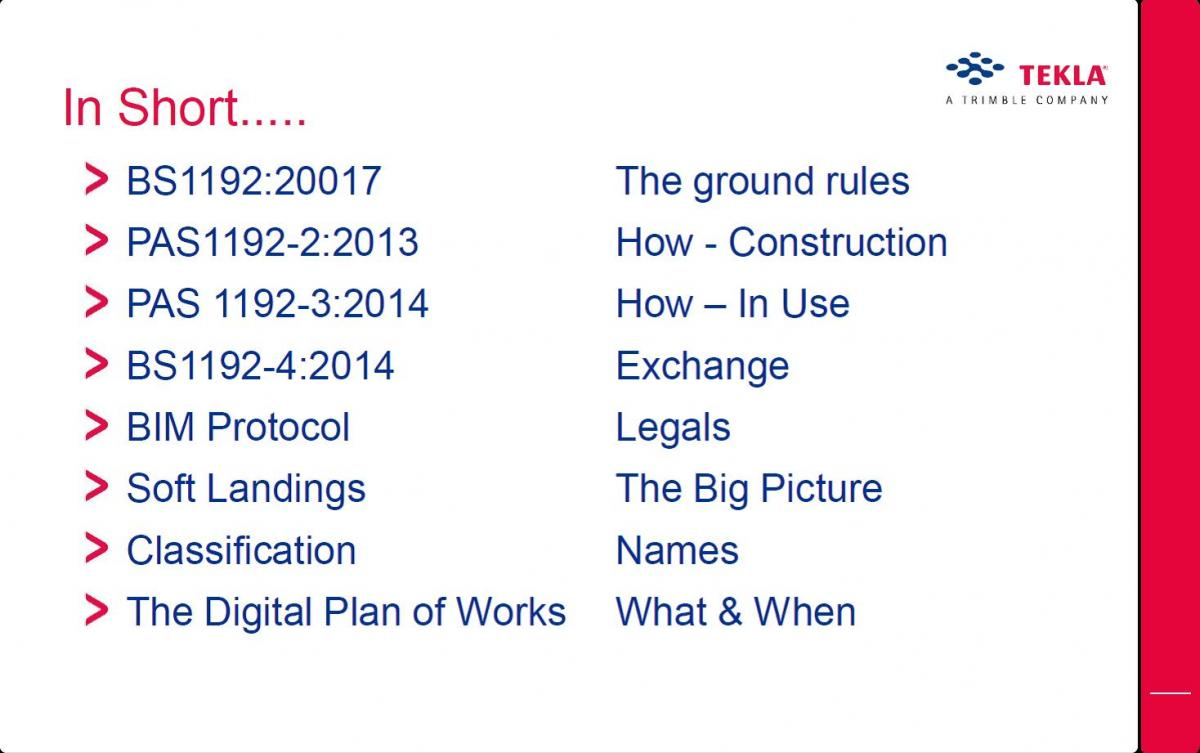
\includegraphics[width=10cm]{./images/BIMsummary.jpg}
	\caption[]{}
	\label{fig:}
\end{figure}
\begin{itemize}
	\item 
\end{itemize}
\end{frame}
\begin{center}\line(1,0){250}\end{center}


\begin{frame}
\frametitle{}
\begin{figure}
	\centering
	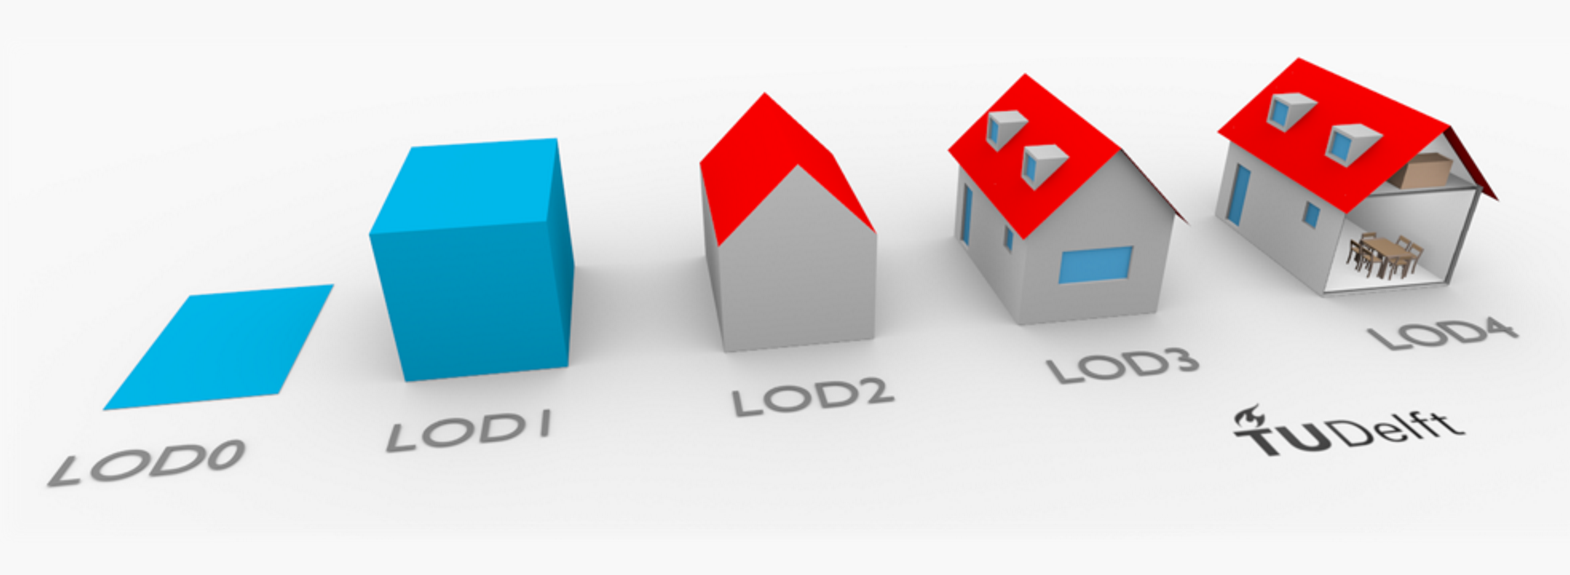
\includegraphics[width=10cm]{./images/TUDelftLODfigure.png}
	\caption[]{}
	\label{fig:}
\end{figure}
\begin{itemize}
	\item 
\end{itemize}
\end{frame}
\begin{center}\line(1,0){250}\end{center}






\section{PAS 1192 Part 2 - Construction}

\begin{frame}
\frametitle{PAS 1192-2:2013}
\begin{figure}
	\centering
	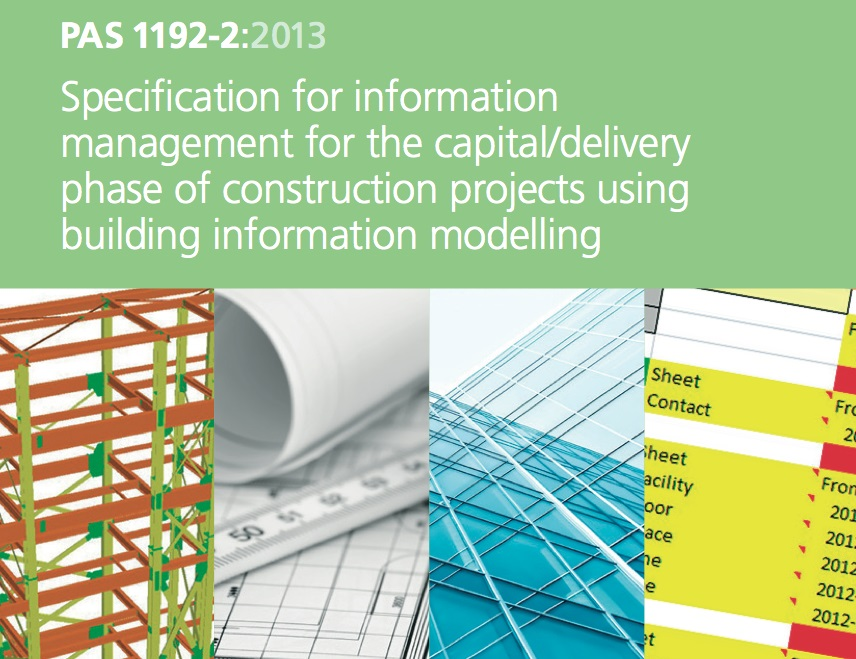
\includegraphics[width=9cm]{./images/Pas1192P2Image.jpg}
	\caption[]{}
	\label{fig:}
\end{figure}
\end{frame}
\begin{center}\line(1,0){250}\end{center}


\begin{frame}
\frametitle{Overview}
\begin{figure}
	\centering
	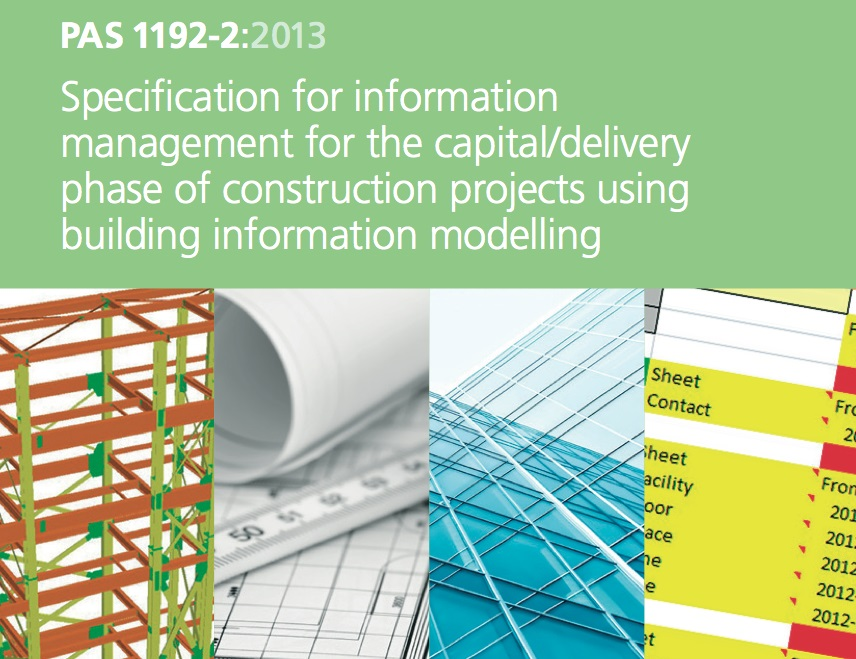
\includegraphics[height=1.5cm]{./images/Pas1192P2Image.jpg}
\end{figure}
\begin{itemize}
	\item Currently in Revision (Sept 2017).
	\item Deals with build-stage requirements
	\item Build Stage requirements should be driven by Operations stage requirements. 
\end{itemize}
\end{frame}
\begin{center}\line(1,0){250}\end{center}


\begin{frame}
\frametitle{Core Principles}
\begin{figure}
	\centering
	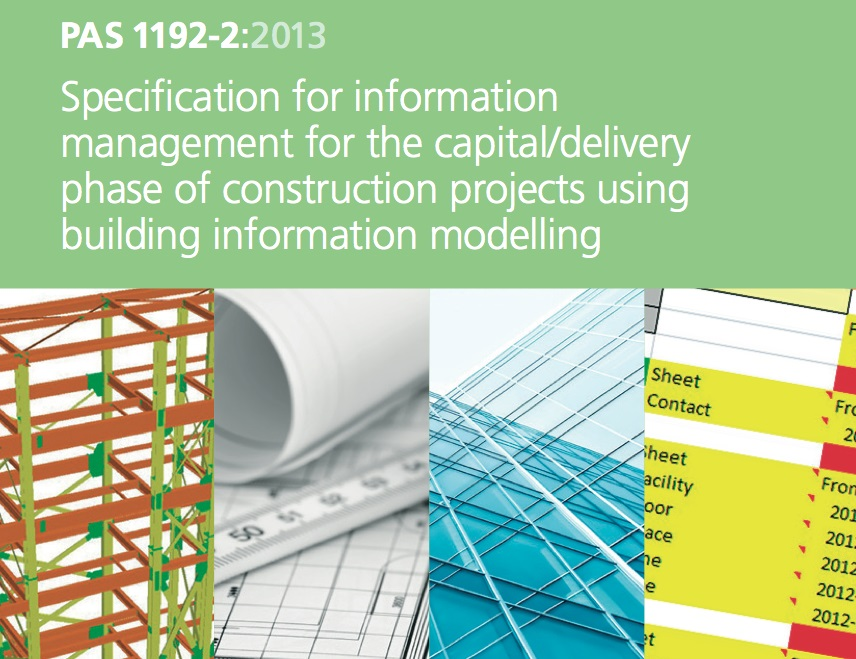
\includegraphics[height=1.5cm]{./images/Pas1192P2Image.jpg}
\end{figure}
\begin{itemize}
	\item Originators produce information in the models they control
	\item There must be a clear definition of information requirements
	\item The BIM approach is evaluated before contract award; and forms part of the contract deliverables
	\item BIM Execution Plan (BEP) is developed by the contractor/supplier
	\item Single, Shared Environment for Data, known as the Common Data Environment (CDE)
	\item Standard Processes and Procedures are applied
\end{itemize}
\end{frame}
\begin{center}\line(1,0){250}\end{center}




\begin{frame}
\frametitle{Core Process}
\begin{figure}
	\centering
	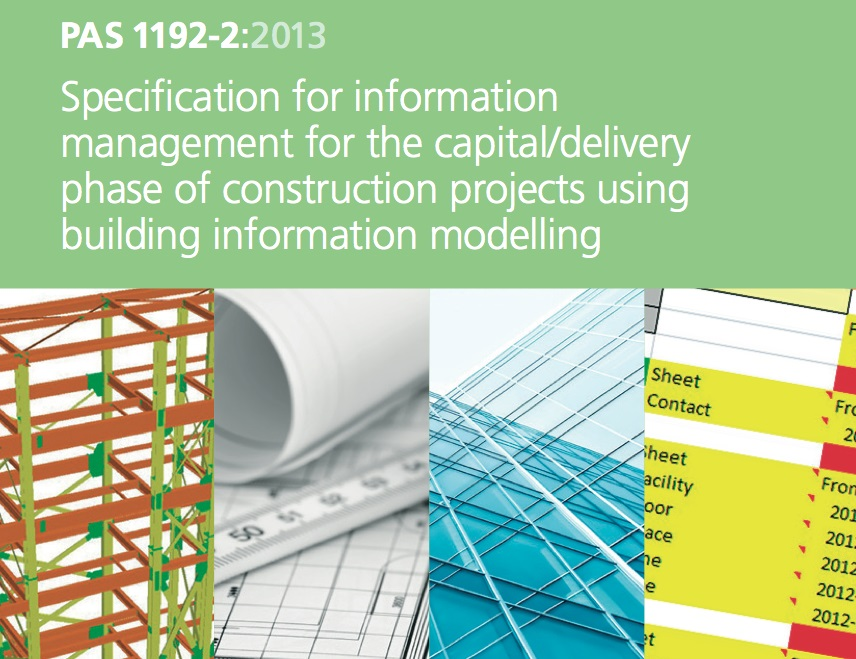
\includegraphics[height=1.5cm]{./images/Pas1192P2Image.jpg}
\end{figure}
\begin{enumerate}
	\item High Level Information Requirement are developed by the client
	\item Plain Language Questions (PLQs) are developed to broaden scope of information required
	\item All stakeholders should develop their own PLQs
	\item PLQ's are amalgamated and turned into specific information requirements
	\item Tender stage client document is the Employers Information Requirements (EIR)
	\item The EIR is responded to by the Contractor in the form of a BIM Execution Plan (BEP)
\end{enumerate}
\end{frame}
\begin{center}\line(1,0){250}\end{center}





\begin{frame}
\frametitle{EIR key considerations}
\begin{itemize}
	\item How will data be organised, stored and protected
	\item How will information be managed and controlled
	\item How will H \& S data be managed
	\item Usage constraints: filesize, storage capacity, bandwidth
	\item Project origin point; physical and data representations
	\item Data formats: Fileformats, and/or data structure
\end{itemize}
\end{frame}
\begin{center}\line(1,0){250}\end{center}


\begin{frame}
\frametitle{Plain Language Questions (PLQs)}
\begin{itemize}
	\item High level, common questions, associated with project or operational requirements.
	\item They should be linked to project gate points.
	\item Project stage will dictate type and the granularity of the questions.
	\item Example Questions from NBS see: \href{https://www.thenbs.com/BIMTaskGroupLabs/questions.html}{https://www.thenbs.com/BIMTaskGroupLabs/questions.html}
	\begin{itemize}
		\item Has a method for measuring energy in use and CO2 emissions been incorporated into the design?
		\item Does the design meet the FM’s needs e.g. access, adaptability, cost, information on the basis of design, accommodation etc.?
	\end{itemize}
	\item NBS examples are too high level to be of real value.	
\end{itemize}
\end{frame}
\begin{center}\line(1,0){250}\end{center}



\begin{frame}
\frametitle{Employers Information Requirements (EIR)}
\begin{itemize}
	\item Key requirement of tender documentation.
	\item States, in clear terms, what information is required from the contractor, and the format the information is to be provided in.
	\item Contractor/Supplier responds with a BIM Execution Plan at tender stage, and the required information during the project delivery.
	\item Authors should write in terms of deliverables, the BEP will how the deliverable is achieved.
\end{itemize}
\end{frame}
\begin{center}\line(1,0){250}\end{center}



\begin{frame}
\frametitle{EIR Requirements}
Suppose there are 4 lifts in a building, One would expect that the following would be in the EIR
\begin{itemize}
	\item Manufacturer, Model, Installation Date,
	\item Energy consumption, warranty and service interval
	\item Capacity, Car dimensions, shaft dimensions,
	\item Connected Elec Panel, Fire Panel, Telecoms Panel, etc. 
\end{itemize}
The majority of requirements will typically transfer from project to project.
\end{frame}
\begin{center}\line(1,0){250}\end{center}



\begin{frame}
\frametitle{EIR and Supply Chain}
\begin{itemize}
	\item It is expected that elements of the EIR will be delegated by main contractors to sub contractors
	\item It is also expected that main contractors will add their own reqirements before letting a subcontract.
	\item eg contractors will typically request additional information, such as Weight, Delivery Date, Storage requirements, etc.
\end{itemize}
\end{frame}
\begin{center}\line(1,0){250}\end{center}


\begin{frame}
\frametitle{Supply Chain Management}
\begin{itemize}
	\item The BIM workflow depends on the supply chain being able to meet the EIR
	\item Nor all supply chain entities have the capability or capacity to deliver in a BIM manner
	\item This aspect is one of the biggest barriers to BIM implementation
	\item Supplier assessment is critical for success.  CPIx has a template to assist in this.  see \href{http://www.cpic.org.uk/cpix/cpix-bim-execution-plan/}{http://www.cpic.org.uk/cpix/cpix-bim-execution-plan/}
\end{itemize}
\end{frame}
\begin{center}\line(1,0){250}\end{center}


\section{PAS 1192 Part 3 - Operations}







\section{Uniclass 2015}


\section{PAS 1192 Part 4 - COBie}



\section{PAS 1192 Part 5 - Security}




\section{PAS 1192 Part 6 - Health & Safety}




\section{PAS 1192 Part 7 - Construction Information}



\end{document}

